\documentclass[twocolumn]{el-author}
\pagestyle{plain}

\usepackage{amsmath,amssymb,amsthm,mathtools}
\usepackage[linesnumbered, ruled]{algorithm2e}
\usepackage[final]{microtype}
\usepackage[final]{hyperref}
\usepackage[inline]{enumitem}
\usepackage{subcaption}

% DEBUG
\usepackage{lipsum}
\DeclareMathOperator*{\argmin}{arg\,min}
\DeclareMathOperator*{\argmax}{arg\,max}

\def\R{\mathbb{R}}
\def\N{\mathbb{N}}

\newtheorem{observation}{Observation}
\newtheorem{lemma}{Lemma}
\newtheorem{theorem}{Theorem}
\usepackage{tikz}
\usetikzlibrary{
	arrows,
	arrows.meta,
	calc,
	graphs,
	patterns,
	positioning,
	shapes,
	decorations.pathmorphing,
}

%DEFAULT STYLE
\tikzset{default style/.style={
	>=Stealth, 
	on grid, 
	auto, 
	thick,
}}

% NODE
\tikzset{default node/.style={
	draw, 
	circle,
	inner sep=0mm,
	minimum size=5mm,
	very thick,
	font=\small,
	black!70,
}}

% LABELS
\tikzset{label/.style={
	draw=none,
	sloped,
}}

\tikzset{label above/.style={
	label,
	midway,
	above=-1mm,
}}

\tikzset{label below/.style={
	label,
	midway,
	below=-1mm,
}}


\title{Paper}

\date{}

\begin{document}
\title{\titletext}

\author{
Gilad Kutiel
\\
Department of Computer Science, Technion, Haifa, Israel
\\
gkutiel@cs.technion.ac.il
}


\abstract{
Given an undirected graph $G = (V, E)$ and a weight function $w:E \to \R$, 
the \Problem{} problem asks to find a minimum weight sub-tree of $G$, 
$T = (U, F)$, such that every $v \in V \setminus U$ is adjacent to at least one 
vertex in $U$.
The special case when the weight function is uniform is known as the 
\textsc{Minimum Connected Dominating Set} problem.

Given an undirected graph $G = (V, E)$ with some subsets of vertices called groups,
and a weight function $w:E \to \R$,
the \textsc{Group Steiner Tree} problem is to find a minimum weight sub-tree
of $G$ which contains at least one vertex from each group. 

In this paper we show that the two problems are equivalent
from the perspective of approximability.
This improves upon both the best known approximation algorithm and the best 
inapproximability result for the \Problem{} problem.
}

\date{}

\maketitle

\section{Introduction}
An introduction \cite{surlin1976all} with
\begin{enumerate*}
\item algorithm
\item sub figure
\item inline list
\end{enumerate*} 

\begin{algorithm}[H]
	\KwData{this text}
	\KwResult{how to write algorithm with \LaTeX2e }
	initialization\;
	\While{not at end of this document}{
		read current\;
		\eIf{understand}{
			go to next section\;
			current section becomes this one\;
		}{
			go back to the beginning of current section\;
		}
	}
\caption{How to write algorithms}
\end{algorithm}

\begin{figure}[ht]
\begin{subfigure}[b]{.4\textwidth}
	\centering
	
\begin{tikzpicture}
	\fill[red] (0,0) circle (1cm);
	\end{tikzpicture}
	\caption{a circle}
\end{subfigure}
\hfill
\begin{subfigure}[b]{.4\textwidth}
	\centering
	
\begin{tikzpicture}
	\fill[blue] (0,0) rectangle (4,4);
	\end{tikzpicture}
	\caption{a square}
\end{subfigure}
\end{figure}

\lipsum[1-2]

\section{\Problem{}}
Recall that instance of \ProbGroup{} is a tuple $(G, w, S, \mathcal{G})$,
where $G = (V, E)$ is an undirected graph, $w:E \to \mathcal{R}$ is a weight function, 
$S \subseteq V$ is a set of terminals, and $\mathcal{G} \subseteq 2^S$ is a family of 
groups of terminals.
A Steiner group tree of is a sub-tree of $G$, $T = (U, F)$
such that $g \cap U \neq \emptyset$ for each $g \in \mathcal{G}$.
The cost of such tree is $\sum_e \in F w(e)$.
Given an instance of \ProbGroup{} we are looking for a minimum cost Steiner group tree
of $G$.

In this section we show that \Prob{} is equivalent to \ProbGroup{} from 
approximation perspective, 
that is every approximation algorithm to one problem yields the same approximation 
ratio for the other problem.
To show this we introduce approximation preserving reductions from \Prob{} to \ProbGroup{}
and vice-versa. 


	\subsection{\texorpdfstring{\Prob{} $\leq_p$ \ProbGroup{}}{}}
	We start by showing an approximation-preserving reduction from \Prob{} to
\ProbGroup{}.
Given an instance of \Prob{}, $(G, w)$, where $G = (V, E)$, 
we define an instance of \ProbGroup{},
$(G, w, V, \mathcal{G})$.
We now have to define $\mathcal{G}$: for each vertex $v \in V$ we define 
$g_v \in \mathcal{G}$ to be $\{v\} \cup N(v)$.

\begin{figure}
\begin{center}
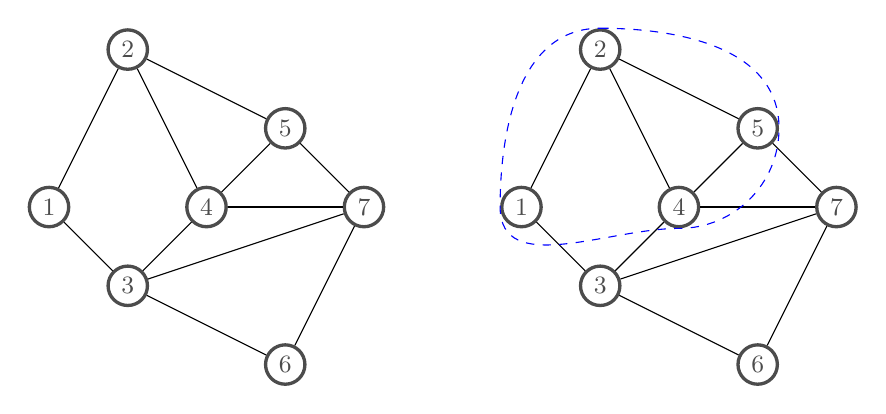
\begin{tikzpicture}[every node/.style={default node}]
\foreach[count=\i] \x \y in {
	0/0
	,1/2,1/-1
	,2/0
	,3/1,3/-2
	,4/0
}{
	\node(\i) at(\x,\y) {\i};
}

\foreach \u \v in {
	1/2,1/3%
	,2/4,2/5%
	,3/4,3/6,3/7%
	,4/5,4/7%
	,5/7%
	,6/7%
}{
	\draw (\u) -- (\v);
}

\begin{scope}[xshift=6cm]
\foreach[count=\i] \x \y in {
	0/0
	,1/2,1/-1
	,2/0
	,3/1,3/-2
	,4/0
}{
	\node(\i) at(\x,\y) {\i};
}

\foreach \u \v in {
	1/2,1/3%
	,2/4,2/5%
	,3/4,3/6,3/7%
	,4/5,4/7%
	,5/7%
	,6/7%
}{
	\draw (\u) -- (\v);
}
\end{scope}

\draw[dashed, blue]
(2.north) to[out=0,in=90]
(5.east) to[out=-90,in=0]
(4.south) to[out=180,in=-90]
(1.west) to[out=90,in=180]
(2.north)
;

\end{tikzpicture}
\end{center}
\caption{\label{fig:prob-leq-group}
From left to right:
a) A \Prob{} instance, weights are omitted.
b) A corresponding \ProbGroup{} instance on the same weighted graph.
For each vertex $v$ we define a group
that contains its neighborhood to ensure that in any group Steiner tree there is at least
one vertex that dominate $v$.
$g_2$ is marked in the figure with a dashed blue line.  
}
\end{figure}

\begin{claim}
Any dominating tree, $T$, in $(G, w)$ is a feasible group Steiner tree in $(G, w, V, \mathcal{G})$.
\end{claim}

\begin{proof}
Assume for contradiction that $T$ is not feasible group Steiner tree, that is, there is 
a group $g_v$ such that none of the vertices in $g_v$ is spanned by $T$, that is $v$
is not in $T$ nor any of its neighbors and thus $T$ is not a dominating tree - contradiction. 
\end{proof}
 
	\subsection{\texorpdfstring{\Prob{} $\geq_p$ \ProbGroup{}}{}}
	We now show an approximation-preserving reduction from \ProbGroup{} to
\Prob{}.
Given an instance of \ProbGroup{}, $(G, w, S, \mathcal{G})$, where $G = (V, E)$, 
we define an instance of \Prob{},
$(G', w')$ where $G' = (V', E')$.


\begin{figure}
\begin{center}
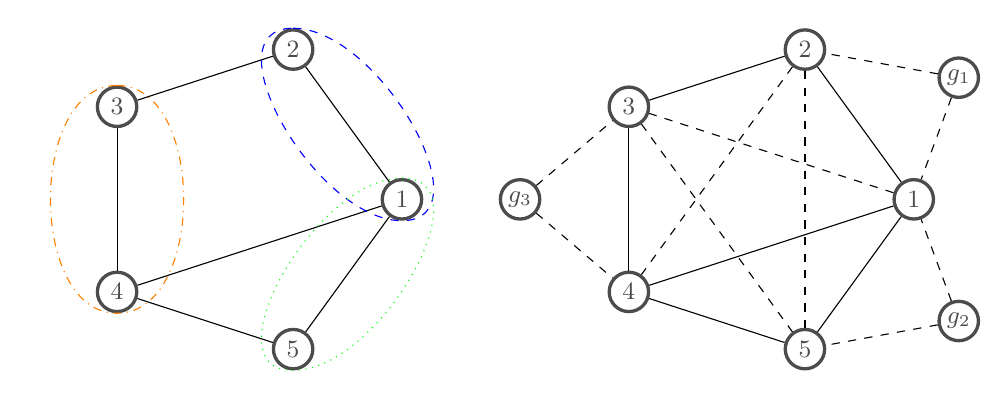
\begin{tikzpicture}[every node/.style={default node}]
\foreach[count=\i] \a in {0,72,...,288}{
	\node(\i) at(\a:2) {\i};
}

\foreach \u \v in {
	1/2,2/3,3/4,4/1,4/5,5/1%
}{
	\draw (\u) -- (\v);
}

\draw[dashed, blue]
(2.north) to[out=0,in=0]
(1.south) to[out=180,in=180]
(2.north)
;

\draw[dotted, green]
(1.north) to[out=0,in=0]
(5.south) to[out=180,in=180]
(1.north)
;

\draw[dash dot, orange]
(3.north) to[out=0,in=0]
(4.south) to[out=180,in=180]
(3.north)
;

\begin{scope}[xshift=65mm]
\foreach[count=\i] \a in {0,72,...,288}{
	\node(\i) at(\a:2) {\i};
}

\foreach \u \v in {
	1/2,2/3,3/4,4/1,4/5,5/1%
}{
	\draw (\u) -- (\v);
}

\node(g1) at(31:3){$g_1$};
\node(g2) at(-31:3){$g_2$};
\node(g3) at(180:3){$g_3$};

\foreach \u \v in {
	1/3%
	,2/4,2/5%
	,3/5%
	%
	,g1/1,g1/2%
	,g2/1,g2/5%
	,g3/3,g3/4%
}{
	\draw[dashed] (\u) -- (\v);
}
\end{scope}

\end{tikzpicture}
\end{center}
\caption{\label{fig:prob-geq-group}
From left to right:
a) An instance of \ProbGroup{} (weights are omitted), 
groups are marked by a dashed blue and dotted green lines respectively.  
b) A corresponding \Prob{} instance: we add a vertex for each group and connect it 
with infinity weighted edges to all terminals in the group.   
}
\end{figure}

\begin{claim}
\end{claim}

\begin{proof}
\end{proof}
 

\section{\ProblemStar{}}
In this section we consider the \ProblemStar{} problem, 
that is the \Problem{} problem when restricted to stars, i.e.
given an undirected weighted graph $(G, w)$ find a 
minimum weight dominating sub-star (a tree with diameter at most 2).
We start by showing that this problem cannot be approximated 
within $c\log n$ for some $c > 0$ unless $P = NP$.
Then we show how to reduce the problem to a set cover instance to achieve a 
$O(\log n)$-approximation algorithm.  
	\subsection{Hardness}
	We show an approximation preserving reduction from the \ProblemDom{} problem (\ProbDom)
to \ProblemStar{}.
Given an (unweighted) instance of \ProbDom{} $G = (V, E)$ we create an instance of \ProbStar{}
$(G', w)$ where $G' = (L \cup R \cup {c}, E' \cup \{c\} \times L$).
\begin{description}
\item[L] - $\{v_l : v \in V\}$
\item[R] - $\{v_r : v \in V\}$
\item[E'] - $\{u_lv_r : uv \in E\}$
\end{description}
We also set $w(e) = \infty$ for every $e \in E'$ and $w(cv_l) = 1$ for every $v_l \in L$.
Figure~\ref{fig:star-hardness} depicts this transformation.
Clearly the above transformation can be done in polynomial time,
The following two claims show that this is an approximation preserving reduction:

\begin{figure}
\begin{center}
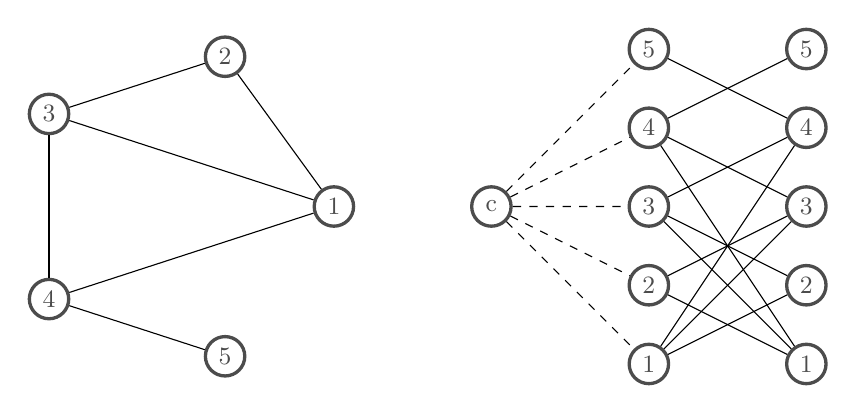
\begin{tikzpicture}[every node/.style={default node}]
\foreach[count=\i] \a in {0,72,...,288}{
	\node(\i) at(\a:2) {\i};
}

\foreach \u \v in {
	1/2,2/3,3/4,4/1,4/5,3/1%
}{
	\draw (\u) -- (\v);
}

\node(c) at(4,0) {c};

\begin{scope}[xshift=6cm, yshift=-3cm]
\foreach \i in {1,...,5}{
	\node(l\i) at(0,\i) {\i};
	\node(r\i) at(2,\i) {\i};
}


\foreach \u \v in {
	1/2,2/3,3/4,4/1,4/5,3/1%
}{
	\draw (l\u) -- (r\v);
	\draw (r\u) -- (l\v);
}

\foreach \i in {1,...,5}{
	\draw[dashed] (c) -- (l\i);
}
\end{scope}
\end{tikzpicture}
\end{center}
\caption{\label{fig:star-hardness}
From left to right:
a) An instance of \ProbDom{} (unweighted graph)
b) The corresponding instance of \ProbStar{}, 
the weight on the original edges (solid black) is infinity 
and the weight on the new edges is 1. 
}
\end{figure} 

\begin{claim}
If $D$ is a dominating set in $G$ then 
$S = (\{c\} \cup \{v_l : v \in D\}, \{cv_l: v \in D\})$ 
is a dominating star in $G'$ that weigh $|D|$. 
\end{claim}

\begin{proof}
$S$ weights $D$ by the definition of $G'$ and $S'$.
Assume for contradiction that it is not a dominating star and let $v$ be a non dominated 
vertex then $v$ is also not dominated in $G$ under $D$ - contradiction.
\end{proof}

\begin{claim}
If $S = (U, F)$ is a dominating star in $G'$ of weight $k < \infty$ 
then $\{v : v_l \in U \setminus \{c\}\}$ is a dominating set in $G$ of size $k$.
\end{claim}

\begin{proof}
Observe that any star that contains more than 3 vertices must be centered at $c$ or otherwise
its weight is infinity.
Thus the leaf of the star dominate all vertices in $R$, by construction, this mean that the
corresponding vertices in the original graph dominate all other vertices.
\end{proof}
	\subsection{\texorpdfstring{$\log n$-Approximation}{log(n)-Approximation}}
	We now show how to reduce \ProbStar{} to an instance of the \ProblemSetCover{} problem
(\ProbSetCover{}) in order to obtain a $O(\log n)$-approximation algorithm.
This is the best one can hope for if $P \neq NP$.

Without loss of generality, we assume that the center of the dominating star is known,
or otherwise we can solve the problem for every vertex in the graph assuming it is 
the center.  
Given an undirected weighted graph $(G, w)$ and a the center of the dominating star
$c \in V$ we create the following an instance of \ProbSetCover{} 
$(U, \mathcal{S}, w')$ as follow:
\begin{description}
\item[$U$] - $V \setminus N(c)$
\item[$\mathcal{S}$] - $\{S_v : cv \in E\}$
\item[$S_v$] - $N(v) \cap U$
\item[$w'$] - $w'(S_v) = w(cv)$ 
\end{description}


\begin{claim}
If $S = (c, L)$ is a dominating star in $G$ then 
$\mathcal{C} = \{S_v : v \in L\}$ is a set cover in $(U, \mathcal{S}, w')$,
moreover, $w(S) = w'(\mathcal{C})$.  
\end{claim}

\begin{proof}
$w(S) = w'(\mathcal{C})$ by construction.
Now, assume for contradiction that $\mathcal{C}$ is not a set cover and let $v$
be an uncover element then $v$ is also not dominated by $S$ - contradiction.
\end{proof}

\begin{claim}
If $\mathcal{C}$ is a set cover in $(U, \mathcal{S}, w')$ 
then $S = (c, \{v : S_v \in \mathcal{C}\})$ is a dominating star in $G$,
moreover, $w(S) = w'(\mathcal{C})$.  
\end{claim}

\begin{proof}
$w(S) = w'(\mathcal{C})$ by construction.
Now, assume for contradiction that $S$ is not a dominating star and let $v$
be an undominated vertex then $v$ is also uncovered by $\mathcal{C}$ - contradiction.
\end{proof}

\section{\ProblemPath{}}
We show that the \ProblemPath{} problem (\ProbPath{}) cannot be approximated at all
unless $P = NP$.
We show a reduction from the \ProblemHam{} problem (\ProbHam{}).
In \ProbHam{} we are given an undirected graph $G = (V, E)$ and we are 
asked to decide if there is an Hamiltonian path 
(a simple path traversing all the vertices in $V$) in $G$ or not.
\ProbHam{} is one of the classical NP-hard problems.

Given an instance of \ProbHam{}, $G = (V, E)$, we define an instance of \ProbPath{},
$(G', w)$, where $G' = (V \cup \{v' : v \in V\}, E \cup \{vv' : v \in V\})$.
We set $w(e) = 0$ for every edge $e \in E$ and set $w(e) = \infty$ otherwise.
Figure~\ref{fig:hamiltonian} depicts this transformation.  
We now claim that any (multiplicative) approximation algorithm for \ProbPath{}
can solve \ProbHam{}.
Let $G$ be an instance of (decision problem) \ProbHam{}, 
and denote by $A(G', w)$ the value of (approximation) algorithm, $A$, 
on the corresponded \ProbPath{} instance, then:

\begin{claim}
$A(G', w) = 0 \iff G \in \ProbHam{}$. 
\end{claim} 

\begin{proof}
Let $P$ be a dominating path in $(G', w)$ with value 0, 
then it uses only edges of $E$, moreover $P$ is an hamiltonian path in $G$ or otherwise
there is a vertex $v'$ that is not dominated by $P$.
Now, let $P$ be an hamiltonian path in $G$ then $P$ is a dominating path in $G'$ with value
0, thus, any (multiplicative) approximation algorithm must also find a path value 0.
\end{proof}


\begin{figure}
\begin{center}
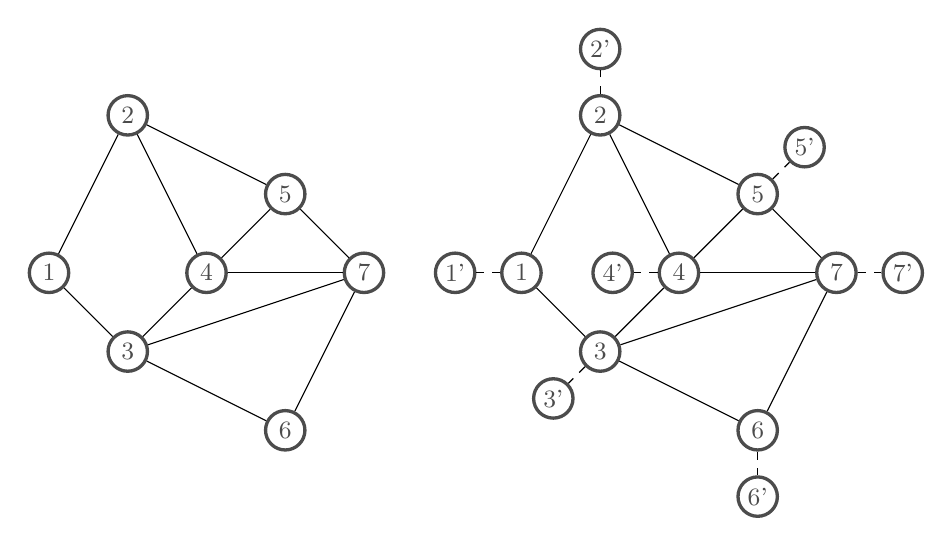
\begin{tikzpicture}[every node/.style={default node}]
\foreach[count=\i] \x \y in {
	0/0
	,1/2,1/-1
	,2/0
	,3/1,3/-2
	,4/0
}{
	\node(\i) at(\x,\y) {\i};
}

\foreach \u \v in {
	1/2,1/3%
	,2/4,2/5%
	,3/4,3/6,3/7%
	,4/5,4/7%
	,5/7%
	,6/7%
}{
	\draw (\u) -- (\v);
}

\begin{scope}[xshift=6cm]
\foreach[count=\i] \x \y in {
	0/0
	,1/2,1/-1
	,2/0
	,3/1,3/-2
	,4/0
}{
	\node(\i) at(\x,\y) {\i};
}

\foreach \u \v in {
	1/2,1/3%
	,2/4,2/5%
	,3/4,3/6,3/7%
	,4/5,4/7%
	,5/7%
	,6/7%
}{
	\draw (\u) -- (\v);
}

\foreach[count=\i] \p in {
	left,above,below left,left,above right,below,right%
}{
	\node(\i')[\p=3mm of \i] {\i'};
	\draw[dashed] (\i) -- (\i');
}
\end{scope}
\end{tikzpicture}
\end{center}
\caption{\label{fig:hamiltonian}
From left to right
a) An instance of the \ProblemHam{} problem.
b) The corresponded \ProblemPath{} instance, 
original edges have zero weight, dashed edges have infinite weight.
}
\end{figure} 

\section{Conclusion}
Our result shows that on general graphs any approximation algorithm for
the \Problem{} problem yields the same approximation result for the 
\ProblemGroup{} problem and vice versa.
This result might give another perspective and maybe shed some light on
the \ProblemGroup{} problem.

We remark, however, that the two problems are not equivalent.
A good example is when the input graph is a tree, \ProbGroup{} is known to 
be as hard to approximate as \ProbSetCover{} even in this case while \Prob{} is 
trivially solvable on trees.
Thus, there is also a place to studying each of the problems on its own for particular 
families of graphs.

\nocite{*}
\bibliographystyle{plain}
\bibliography{main}

\end{document}